\documentclass[letterpaper,12pt,oneside]{article}\usepackage[]{graphicx}\usepackage[]{color}
%% maxwidth is the original width if it is less than linewidth
%% otherwise use linewidth (to make sure the graphics do not exceed the margin)
\makeatletter
\def\maxwidth{ %
  \ifdim\Gin@nat@width>\linewidth
    \linewidth
  \else
    \Gin@nat@width
  \fi
}
\makeatother

\definecolor{fgcolor}{rgb}{0.345, 0.345, 0.345}
\newcommand{\hlnum}[1]{\textcolor[rgb]{0.686,0.059,0.569}{#1}}%
\newcommand{\hlstr}[1]{\textcolor[rgb]{0.192,0.494,0.8}{#1}}%
\newcommand{\hlcom}[1]{\textcolor[rgb]{0.678,0.584,0.686}{\textit{#1}}}%
\newcommand{\hlopt}[1]{\textcolor[rgb]{0,0,0}{#1}}%
\newcommand{\hlstd}[1]{\textcolor[rgb]{0.345,0.345,0.345}{#1}}%
\newcommand{\hlkwa}[1]{\textcolor[rgb]{0.161,0.373,0.58}{\textbf{#1}}}%
\newcommand{\hlkwb}[1]{\textcolor[rgb]{0.69,0.353,0.396}{#1}}%
\newcommand{\hlkwc}[1]{\textcolor[rgb]{0.333,0.667,0.333}{#1}}%
\newcommand{\hlkwd}[1]{\textcolor[rgb]{0.737,0.353,0.396}{\textbf{#1}}}%

\usepackage{framed}
\makeatletter
\newenvironment{kframe}{%
 \def\at@end@of@kframe{}%
 \ifinner\ifhmode%
  \def\at@end@of@kframe{\end{minipage}}%
  \begin{minipage}{\columnwidth}%
 \fi\fi%
 \def\FrameCommand##1{\hskip\@totalleftmargin \hskip-\fboxsep
 \colorbox{shadecolor}{##1}\hskip-\fboxsep
     % There is no \\@totalrightmargin, so:
     \hskip-\linewidth \hskip-\@totalleftmargin \hskip\columnwidth}%
 \MakeFramed {\advance\hsize-\width
   \@totalleftmargin\z@ \linewidth\hsize
   \@setminipage}}%
 {\par\unskip\endMakeFramed%
 \at@end@of@kframe}
\makeatother

\definecolor{shadecolor}{rgb}{.97, .97, .97}
\definecolor{messagecolor}{rgb}{0, 0, 0}
\definecolor{warningcolor}{rgb}{1, 0, 1}
\definecolor{errorcolor}{rgb}{1, 0, 0}
\newenvironment{knitrout}{}{} % an empty environment to be redefined in TeX

\usepackage{alltt}
\usepackage[paperwidth=8.5in,paperheight=11in,top=1in,bottom=1in,left=1in,right=1in]{geometry}
\usepackage{setspace}
\usepackage[colorlinks=true,allcolors=Blue]{hyperref}
\usepackage[usenames,dvipsnames]{xcolor}
\usepackage{indentfirst}
\usepackage{titlesec}
\usepackage{multirow}
\usepackage{booktabs}
\usepackage{graphicx}
\usepackage{verbatim}
\usepackage{rotating}
\usepackage{tabularx}
\usepackage{outlines}
\usepackage{lineno}
\usepackage{array}
\usepackage{times}
\usepackage{cleveref}
\usepackage{acronym}
\usepackage[position=t]{subfig}
\usepackage{paralist}
\usepackage[noae]{Sweave}
\usepackage{natbib}
\usepackage{array}
\usepackage{pdflscape}
\usepackage{bm}
\usepackage{showlabels}
\usepackage{outlines}
\bibpunct{(}{)}{,}{a}{}{,}

% page margins and section title formatting
\linespread{1.5}
\setlength{\footskip}{0.5in}
\titleformat*{\section}{\Large\bf\em}
\titleformat*{\subsection}{\singlespace\large\bf}
\titleformat*{\subsubsection}{\singlespace\normalsize\bf\em}
\titlespacing{\section}{0in}{0in}{0in}
\titlespacing{\subsection}{0in}{0in}{0in}
\titlespacing{\subsubsection}{0in}{0in}{0in}

% cleveref options
\crefname{table}{Table}{Tables}
\crefname{figure}{Fig.}{Figs.}
\renewcommand{\figurename}{Fig.}

% aliased citations
% \defcitealias{FLDEP12}{FLDEP 2012}

% acronyms
\acrodef{AIC}{Akaike Information Criterion}
\acrodef{ARMA}{Autoregressive Moving Average}
\acrodef{chla}[chl-\textit{a}]{chlorophyll \textit{a}}
\acrodef{GAM}{generalized additive models}
\acrodef{RMSE}{root mean square error}
\acrodef{USGS}{US Geological Survey}
\acrodef{WRTDS}{weighted regression on time, discharge, and season}

% macros
% for micrograms per litre
\newcommand{\mugl}{$\mu$g L$^{-1}$}

%knitr options


% get the version based on commit date


% R libs


% get online bib file


\IfFileExists{upquote.sty}{\usepackage{upquote}}{}
\begin{document}

\raggedbottom
% \linenumbers
\raggedright
\urlstyle{same}
\setlength{\parindent}{0.5in}
\renewcommand\refname{References \vspace{12pt}}

\begin{singlespace}
\title{{\bf {\Large Comparison of weighted regression and additive models for trend evaluation of water quality in tidal waters}}}
\author{
  {\bf {\normalsize Marcus W. Beck$^1$, Rebecca Murphy$^2$}}
  \\\\{\textit {\normalsize $^1$ORISE Research Participation Program}}
  \\{\textit {\normalsize USEPA National Health and Environmental Effects Research Laboratory}}
  \\{\textit {\normalsize Gulf Ecology Division, 1 Sabine Island Drive, Gulf Breeze, FL 32561}}
	\\{\textit {\normalsize Phone: 850-934-2480, Fax: 850-934-2401, Email: \href{mailto:beck.marcus@epa.gov}{beck.marcus@epa.gov}}}
  \\\\{\textit {\normalsize $^2$UMCES at Chesapeake Bay Program}}
	\\{\textit {\normalsize 410 Severn Avenue, Suite 112, Annapolis, MD 21403}}
	\\{\textit {\normalsize Phone: 410-267-9837, Fax: 410-267-5777, Email: \href{mailto:rmurphy@chesapeakbay.net}{rmurphy@chesapeakebay.net}}}
  \vspace{1in} 
  \\ Version Date:   Wed Aug 12 07:53:21 2015 -0500
	}
\date{}
\maketitle
\end{singlespace}
\clearpage

\section*{Abstract}

\noindent Long-term monitoring datasets can provide information to interpret the effects of environmental changes or management actions on ecosystem condition.  The ability to link causal effects with potential changes can depend on the chosen method of interpreting trends in the observed data.  Two statistical approaches, \ac{WRTDS} and \acp{GAM}, have recently been used to evaluate long-term trends in chlorophyll time series in estuarine systems.  Both models provide a similar approach to trend analysis by using context-dependent parameters or smoothing functions that vary continuously and have the potential to identify multiple drivers of change.  However, the quantitative capabilities of each model, including descriptions of observed and flow-normalized trends, have not been rigorously compared to determine most appropriate use of each model.  We evaluated \ac{WRTDS} and \acp{GAM} using thirty years of data for a monthly time series of chlorophyll in the Patuxent River Estuary, a well-studied tributary to Chesapeake Bay.  Each model was evaluated based on goodness of fit to the observed data and ability to reproduce flow-normalized trends with simulated data that had statistical properties comparable to the original dataset.  Each model was also evaluated based on concordance of conclusions of water quality changes, and causes thereof, in different time periods.  This information will provide researchers with valuable guidance for using statistical models in trend evaluation, with particular relevance for computational requirements, desired products, and future data needs.  

\noindent \textit{Key words}: chlorophyll, estuary, generalized additive models, Patuxent River Estuary, trend analysis, weighted regression

\clearpage

\acresetall

\section{Introduction}

The interpretation of enviromental trends can have widespread implications for the management of natural resources and can facilitate an understanding of ecological factors that mediate system dynamics.  An accurate interpretation of trends can depend on the chosen method of analysis, and more importantly, its ability to consider effects of multiple drivers on response endpoints that may be particular to the system of interest.  The need to interpret potential impacts of nutrient pollution has been a priority issue for managing aquatic resources \citep{Nixon95}, particularly for estuaries that serve as focal points of human activities and receiving bodies for upstream hydrologic networks \citep{Paerl14}.  Common assessment endpoints for eutrophication in estuaries have included seagrass growth patterns \citep{Steward07}, frequency and magnitude of oxygen depletion in bottom waters \citep{Paerl06}, and trophic network connectivity \citep{Powers05}.  Additionally, chlorophyll concentration provides a measure of the release of phytoplankon communities from nutrient limitation with increasing eutrophication.  Chlorophyll time series have been collected for decades in tidal systems (e.g., Tampa Bay, \citet{TBEP11}; Chesapeake Bay, \citet{Harding94}; datasets cited in \citet{Monbet92,Cloern10}), although the interpration of trends in observed data has been problematic given the inherent variability of time series data. Identifying the response of chlorophyll to different drivers, such as management actions or increased pollutant loads, can be confounded by natural variation from freshwater inflows \citep{Borsuk04b} or tidal exchange with oceanic outflows \citep{Monbet92}.  Seasonal and spatial variability of chlorophyll dynamics (see \citet{Cloern96}) can further complicate trend evaluation, such that relatively simple analysis methods may insufficiently describe variation in long-term datasets \citep{Hirsch14b}.  More rigorous quantitative tools are needed to create an unambiguous characterization of chlorophyll response independent of variation from confounding variables.

% WRTDS and GAMs as novel methods
Recent applications of statistical methods to describe water quality dynamics have shown promise in estuaries, specifically \ac{WRTDS} and \acp{GAM}.  The \ac{WRTDS} method was initially developed to describe water quality trends in rivers \citep{Hirsch10,Hirsch14} and has recently been adapted to describe chlorophyll trends in tidal waters \citep{Beck15}.  A defining characteristic of \ac{WRTDS} is a weighting scheme that fits a continuous set of parameters to the time series by considering the influence of location in the record and contextual flow inputs to the period of interest.  The \ac{WRTDS} model has been used to model pollutant delivery from tributary sources to Chesapeake Bay \citep{Hirsch10,Moyer12,Zhang13}, Lake Champlain \citep{Medalie12}, and the Mississippi River \citep{Sprague11}.  A comparison to an alternative regression-based model for evaluating nutrient flux, ESTIMATOR, suggested that \ac{WRTDS} can produce more accurate trend estimates \citep{Moyer12}. Similarly, \acp{GAM} can be used to describe variation in a response variable as a sum of smoothing functions for different predictors \citep{Hastie90,Wood06}.  In applications to water quality time series, \acp{GAM} are similar to \ac{WRTDS} in that variable effects through time can be described in relation to seasonal or annual changes.  Application of \acp{GAM} to describe eutrophication endpoints in tidal waters have not been as extensive as \ac{WRTDS}, although exploratory analyses have suggested that results are comparable.  Moreoever, \acp{GAM} are particularly appealing because they are less computationally intense and provide more accessible estimates of model uncertainty than \ac{WRTDS}.  Despite the potential for both approaches to characterize system dynamics, the relative merits of each have not been evaluated.  Quantitative comparisons that describe the accuracy of empirical descriptions and the desired products could inform the use of each model to describe long-term changes in ecosystem characteristics.

% goals/objectives
The goal of this study is to provide an empirical description of the relative abilities of \ac{WRTDS} and \acp{GAM} to describe long-term changes in time series of eutrophication response endpoints in tidal waters.  A thirty year time series of monthly chlorophyll observations from the Patuxent River Estuary is used as a common dataset for evaluating each model.  The Patuxent Estuary is a well-studied tributary of the Chesapeake Bay system that has been monitored for several decades with fixed stations along the longitudinal axis.  Two stations were chosen as representative time series that differed in the relative contributions of watershed inputs and influences from the mainstem of the Chesapeake, in addition to known historical events that have impacted water quality in the estuary.  The specific objectives of the analysis were to \begin{inparaenum}[1\upshape)]
\item provide a narrative comparison of the statistical foundation of each model, both as a general description and as a means to evaluate water quality time series,
\item use each model to develop an empirical description of water quality changes at each monitoring station given known historical changes in water quality drivers,
\item evaluate each models's ability to reproduce flow-normalized trends as known components of simulated time series, and
\item compare each technique's ability to describe changes, as well as the differences in the information provided by each. 
\end{inparaenum}
We conclude with recommendations on the most appropriate use of each method, with particular attention given to computational requirements, uncertainty assessment, and potential needs for additional monitoring data.

\section{Methods}

\subsection{Study site and water quality data}

% flow data from Bowie, MD gage


The Patuxent River estuary, Maryland, is a tributary to Chesapeake Bay on the Atlantic coast of the United States (\Cref{fig:map}). The longitudinal axis extends 65 km landward from the confluence with the mesohaline portion of Chesapeake Bay.  Estimated total volume at mean low water is 577 x 10$^6$ m$^3$ and a surface area of 126 x 10$^6$ m$^2$.  The lower estuary (below 45 km from the confluence) has a mean width of 2.2 km and depth of 6 m \citep{Cronin75}, whereas the upper estuary has a a mean width of 0.4 km and mean depth of 2.5 m \citep{Hagythes}.  The lower estuary is seasonally stratified and vertically-mixed in the upper estuary.  A two-layer circulation pattern occurs in the lower estuary characterized by an upper seaward-flowing layer and a lower landward-flowing layer.  A mixed diurnal tide dominates with mean range varying from 0.8 m in the upper estuary to 0.4 m near the mouth \citep{Boicourt98}.  The estuary drains a 2300 km$^2$ watershed that is 49\% forest, 28\% grassland, 12\% developed, and 10\% cropland \citep{Jordan03}.  The \ac{USGS} stream gage on the Patuxent River at Bowie, Maryland measures discharge from 39\% of the watershed.  Daily mean discharge from 1985 to 2014 was 11.0 m$^3$ s$^{-1}$, with abnormally high years occuring in 1996 (annual mean 20.0 m$^3$ s$^{-1}$) and 2003 (annual mean 22.5  m$^3$ s$^{-1}$). 

The Chesapeake Bay Program maintains a continuous monitoring network for the Patuxent at ten fixed stations that cover the salinity gradient from estuarine to tidal fresh (\href{http://www.chesapeakebay.net/}{http://www.chesapeakebay.net/}, \cref{fig:map}).  Water quality samples have been collected since 1985 at monthly or bimonthly intervals and include salinity, temperature, \ac{chla}, dissolved oxygen, and additional dissolved or particulate nutrients and organic carbon.  Seasonal variation in \ac{chla} is observed across the stations with spring and summer blooms occuring in the upper, oligohaline section, whereas primary production is generally higher in the lower estuary during winter months (\cref{fig:chlyrmofl}).  Chlorophyll concentrations are generally lowest for all stations in late fall and early winter.  Periods of low flow are associated with higher chlorophyll concentrations in the upper estuary, whereas the opposite is observed for high flow.  Stations TF1.6 and LE1.2 were chosen as representative time series from different salinity regions to evaluate the water quality models.  Observations at each station capture a longitudinal gradient of watershed influences at TF1.6 to mainstem influences from the Chesapeake Bay at LE1.2.  Long-term changes in chlorophyll have also been related to historical reductions in nutrient inputs following a statewide ban on phosphorus-based detergents in 1984 and wastewater treatment improvements in the early 1990s that reduced point sources of nitrogen \citep{Lung03,Testa08a}.  Therefore, the chosen stations provide unique datasets to evaluate the predictive and flow-normalization abilities of each model given the differing contributions of landward and seaward influences on water quality.

Thirty years of monthly chlorophyll and salinity data from 1986 to 2014 were obtained for stations TF1.6 and LE1.2 from the Chesapeake Bay Program data hub.  All data were vertically integrated throughout the water column for each date to create a representative sample of water quality.  The integration averaged all values after interpolating from the surface to the maximum depth. Observations at the most shallow and deepest sampling depth were repeated for zero depth and maximum depths, respectively, to bound the interpolations within the range of the data.  Daily flow data were also obtained from the \ac{USGS} stream gage station at Bowie, Maryland and merged with the nearest date in the chorophyll and salinity time series.  Initial analyses suggested that a moving-window average of discharge for the preceding five days of each observation provided a better fit to the chlorophyll data.  Both chlorophyll and discharge data were log-transformed.  Censored data were not present in any of the data sets.  Initial quality assurance checks for all monitoring data were conducted following standard protocols adopted by the Chesapeake Bay Program.        

\subsection{Model descriptions}

%How, Similarities, differences, optimal smoothing

\subsubsection{Weighted Regression on Time, Discharge, and Season}

The \ac{WRTDS} method relates a response endpoint, typically a nutrient concentration, to flow and time to evaluate trends in long-term water quality \citep{Hirsch10,Hirsch14}. Recent adaptation of \ac{WRTDS} to tidal waters relates chlorophyll concentration to salinity and time \citep{Beck15}.  The functional form of the model is a simple regression that relates the natural log of chlorophyll ($Chl$) to decimal time ($T$) and salinity ($Sal$) on a sinuisoidal annual time scale (i.e., cyclical variation by year). 
\begin{equation} \label{eqn:funform}
\ln\left(Chl\right) = \beta_0 + \beta_1 T + \beta_2 Sal + \beta_3 \sin\left(2\pi T\right) + \beta_4 \cos\left(2\pi t\right) + \epsilon
\end{equation}
The tidal adaptation of \ac{WRTDS} uses quantile regression models \citep{Cade03} to characterize trends in different conditional distributions of chlorophyll, e.g., the median or 90th percentile. For comparison to \acp{GAM}, the standard \ac{WRTDS} model that characterizes the conditional mean of the response was used.  Mean models require an estimation of the back-transformation bias parameter. This is achieved by accounting for the standard error of residuals for each observation along the time series during back-transformation \citep{Hirsch10}.  Additionally, the \ac{WRTDS} model uses survival regression as a variation of the weighted Tobit model \citep{Tobin58} to account for censored observations beyond the detection limit \citep{Hirsch14}.

The \ac{WRTDS} approach obtains fitted values of the response variable by estimating regression parameters for each unique observation. Specifically, a unique regression model is estimated for each point in the period of observation. Each model is weighted by month, year, and salinity such that a unique set of regression parameters for each observation is obtained. For example, a weighted regression centered on a single observation weights other observations in the same year, month, and similar salinity with higher importance, whereas observations for different months, years, or salinities receive lower importance. This weighting approach allows estimation of regression parameters that vary in relation to observed conditions \citep{Hirsch10}. Optimal window widths can be identified using cross-validation, described below, thats evaluates the ability of the model to generalize results with novel datasets.

Predicted values are based on an interpolation matrix from the unique regressions at each time step. A sequence of salinity values based on the minimum and maximum values for the data are used to predict chlorophyll using the observed month and year based on the parameters fit to the observation. Model predictions are based on a bilinear interpolation from the grid using the salinity and date values closest to observed. Salinity-normalized values are also obtained from the prediction grid that allow an interpretation of chlorophyll trend that is independent of variation related to salinity changes. Normalized predictions are obtained for each observation by collecting the sample of observed salinity values that for the same month throughout all years in the dataset.  These salinity values are assumed to be equally likely to occur across the time series at that particular month. A normalized value for each point in the time series is the average of the predicted values from each specific model based on the salinity values that are expected to occur for each month.

\subsubsection{Generalized Additive Models}

\subsubsection{Selection of model parameters}

The selection of optimal model parameters is a challenge that represents a tradeoff between model precision and ability to generalize to novel datasets.  Weighted regression requires identifying optimal half-window widths, whereas \acp{GAM} requires identifying the optimal degrees of freedom for the smoothing parameter.  Overfitting a model with excessively small window widths or excessive degrees of freedom will minimize prediction error but prevent extrapolation of results to different datasets. Similarly, underfitting a model with large window widths or very few degrees of freedom will reduce precision but will improve the ability to generalize results to different datasets. From a statistical perspective, the optimal model parameters provide a balance between over- and under-fitting.  Both models use a form of cross-validation to identify model parameters that maximize the precision of model predictions with a novel dataset.   

The basic premise of cross-validation is to identify the optimal set of model parameters that minimize prediction error on a dataset that was not used to develop the model.  For \acp{GAM} \citep{Hastie90,Zuur12}...[insert GAMs methods]. Similarly, the tidal adaptation of \ac{WRTDS} used k-fold cross-validation to identify the optimal half-window widths. For a given set of half-window widhts, the dataset was separated into ten disjoint sets, such that ten models were evaluated for every combination of k - 1 training and remaining test datasets. That is, the training dataset for each fold was all k - 1 folds and the test dataset was the remaining fold, repeated k times. The average prediction error of the test datasets across k folds provided an indication of model performance for the given combination of half-window widths.  The optimum window widths were those that provided minimum errors on the test data.  Evaluating multiple combinations of window-widths can be computationally intensive. An optimization function was implemented in R  \citep{Byrd95,RDCT15} to more efficiently evaluate model parameters using a search algorithm.  Window widths were searched using the limited-memory modification of the BFGS quasi-Newton method that imposes upper and lower bounds for each parameter.  The chosen parameters were based on a selected convergence tolerance for the error minimization of the search algorithm.  

\subsection{Comparison of modelled trends}

Separate \ac{WRTDS} and \acp{GAM} were created using the above methods for the chlorophyll time series at TF1.6 and LE1.2.  Initial analyses indicated that model performance could be improved using the flow record to model \ac{chla} at TF1.6 and the salinity record to model \ac{chla} at LE1.2.  For each model and station, a predicted and flow-normalized (hereafter flow-normalized refers to both flow and salinity) time series was obtained for comparison.  The results were compared using several summary statistics that evaluated both the predictive performance to describe observed chlorophyll and direct comparisons between the models.  Emphasis was placed on agreement between predictions and observed values, rather than uncertainty associated with parameter estimates.  As of writing, methods for estimating confidence intervals of \ac{WRTDS} have not been fully developed for application to \ac{WRTDS} in tidal waters.  In addition to simple visual evaluation of trends over time and bivariate scatterplot comparisons, summary statistics used to compare model predictions to observed \ac{chla} included explained variance ($R^2$) and \ac{RMSE}.  Model results were compared directly using average differences and evaluation of a regression fit for the results comparing each model to a line with intercept of zero and slope of one.  Deviation of the slope of the regression either greater or less than one indicated potential bias for a particular model as under- or over-predicting relative to the other.  For all comparisons, \ac{RMSE} comparing each model's predictions to observed \ac{chla} was defined as:
\begin{equation}
RMSE = \sqrt {{\frac{{\sum\limits_{{i = 1}}^n {{{\left( {{Chl_i} - {{\hat{Chl}}_i}} \right)}^2}} }}{{n}}}}
\end{equation}
where $n$ is the number of observations for a given evaluation, $Chl_i$ is the observed value of \ac{chla} for observation $i$, and ${\hat{Chl}}_i$ is the predicted value of \ac{chla} for observation $i$.  \ac{RMSE} values closer to zero represent model predictions closer to observed.  Similarly, average difference between models as a percentage was defined as:
\begin{equation}
\textrm{Average difference} = \left(\frac{\sum\limits_{i = 1}^n \hat{Chl}_{WRTDS,\,i} - \sum\limits_{i = 1}^n \hat{Chl}_{GAM,\,i}}{\sum\limits_{i = 1}^n \hat{Chl}_{GAM,\,i}}\right) * 100
\end{equation}
where $\hat{Chl}_{WRTDS,\,i}$ and $\hat{Chl}_{GAM,\,i}$ are the predicted values of \ac{chla} for each model at observation $i$.  Positive values indicate that \ac{WRTDS} provided larger predictions than \acp{GAM} on average, whereas the opposite is true for negative values \citep{Moyer12}. 

The statistical comparisons described above were conducted for the entire time series at each station to evaluate overall performance.  Different time periods were also evaluated to identify potential temporal variation in results, which included a comparison of results by annual and seasonal aggregations and periods with different levels of flow.  Annual and seasonal aggregations shown in \cref{fig:chlyrmofl} were evaluated between the models, in addition to evaluating the models at different levels of flow defined by the quartile distributions (min--25\%, 25\%--median, median--75\%, and 75\%--max) relevant to each station.  Flow-normalized time series were compared similarly but only between the models because the true flow-independent component of the observed data is not known and can only be empirically estimated.  As described below, an evaluation of the flow-normalized data was primarily accomplished using simulated datasets with known components that were independent of discharge.  

% Error histograms (see page 14 in Moyer) - we can test for significant differences in the errors using a two-sided t-test. \\
% Indications of change - direction/magnitude of trends by different time periods

\subsection{Comparison of flow-normalized trends}

The relative abilities of each model to characterize flow or salinity-normalized trends in chlorophyll were evaluated using simulated datasets with known components.  This approach was used because the flow-independent component of chlorophyll is typically not observed in raw data such that the true signal must be empirically estimated.  Accordingly, the ability of each model to isolate the flow-normalized trend cannot be evaluated with reasonable certainty unless the true signal is known.  Simulated time series of observed chlrophyll ($Chl_{obs}$) were created as additive components related to flow ($Chl_{flo}$, analogous to salinity) and a flow-independent biological component of chlorophyll ($Chl_{bio}$):
\begin{equation} \label{chlobs}
Chl_{obs} = Chl_{flo} + Chl_{bio}
\end{equation}
A distinction between $Chl_{flo}$ and $Chl_{bio}$ is that the former describes variation in the observed time series with changes in discharge (e.g., concentration dilution with increased flow) and the latter describes a true, desired measure of chlorophyll in the water column that is directly linked to primary production.  The biological component of chlorophyll is comparable to an observation in a closed system that is not affected by flow and is the time series that is estimated by flow-normalization with \ac{WRTDS} and \acp{GAM}.

The simulated time series was based on a stochastic model derived from actual flow and water quality measurements to ensure the statistical properties were comparable to existing datasets.  This approach allowed us to evaluate \acp{GAM} and \ac{WRTDS} under different sampling regimes (e.g., monthly rather than daily), while ensuring the simulated datasets had statistical properties that were consistent with known time series. Daily flow observations were obtained from the \ac{USGS} stream gage station 01594440 near Bowie, Maryland (38$^{\circ}$57$'$21.3$''$N, 76$^{\circ}$41$'$37.3$''$W) from 1985 to 2014.  Daily chlorophyll records were obtained from the Jug Bay station (38$^{\circ}$46$'$50.6$''$N, 76$^{\circ}$42$'$29.1$''$W) of the Chesapeake Bay Maryland National Estuarine Research Reserve.  Daily chlorophyll concentrations were estimated from fluorescence values that did not include blue-green algae blooms.  Our primary concern was simulating chlorophyll concentrations at monthly or bimonthly timesteps such that taxa-specific concentrations on a daily time step were not relevant.

Four time series were estimated or simulated from the actual datasets to create the complete, simulated time series:\begin{inparaenum}[1\upshape)]
\item estimated discharge as a stationary seasonal component ($\hat{Q}_{seas}$),
\item simulated error structure from the residuals of the seasonal discharge model ($\varepsilon_{Q,\,sim}$), 
\item estimated chlorophyll independent of discharge as a stationary seasonal component ($\hat{Chl}_{seas}$), and
\item simulated error structure from the residuals of the seasonal chlorophyll model ($\varepsilon_{Chl,\,sim}$).
\end{inparaenum}
Unless otherwise noted, chlorophyll and discharge are in ln-transformed units.  Each of the four components was used to simulate the components in \cref{chlobs}:
\begin{equation} \label{chlflo}
Chl_{flo} = I\left(\hat{Q}_{seas} + \sigma\cdot\varepsilon_{Q,\,sim}\right)
\end{equation}
\begin{equation} \label{chlbio}
Chl_{bio} = \hat{Chl}_{seas} + \sigma\cdot\varepsilon_{Chl,\,sim}
\end{equation}
The estimated flow time series within the parentheses, $\hat{Q}_{seas} + \sigma\cdot\varepsilon_{Q,\,sim}$, is floored at zero to simulate an additive effect of increasing flow on $Chl_{obs}$.  Although the actual relationship of water quality measurements with flow is more complex, we assumed that a simple addition was sufficient for the simulations where the primary objective was to create an empirical and linear link between flow and chlorophyll. Moreover, the vector $I$ (where $0 \leq I \leq 1$) can be manually changed to represent an independent effect of flow based on the desired simulation.  For example, a flow effect that changes from non-existent to positive throughout the period of observation can be simulated by creating a vector ranging from zero to one. For the simulated $Chl_{bio}$ time series, the seasonal and error components were characterized using the daily time series at Jug Bay that likely included an effect of flow in the observed data.  For the simulated models, we assumed that the actual flow effect was part of the seasonal component to obtain an accurate estimate of the error component that was independent of both flow and season.  Methods for estimating each of the components in \cref{chlflo,chlbio} are described in detail below. 

First, a model for simulating flow-related chlorophyll (\cref{chlflo}) was estimated from the stream gage data as the additive combination of a stationary seasonal component and serially-correlated errors:
\begin{equation} \label{qseas}
Q_{seas} = \beta_0 + \beta_1 \sin\left(2\pi T\right) + \beta_2 \cos\left(2\pi T\right)
\end{equation}
\begin{equation} \label{qerr}
\varepsilon_{Q} = Q_{seas} - \hat{Q}_{seas}
\end{equation}
A seasonal model of flow was estimated using linear regression for time, $T$, on an annual sinusoidal period (\cref{qseas}).  The residuals from this regression, $\varepsilon_{Q}$ (\cref{qerr}), were used to estimate the structure of the error distribution for simulating the stochastic component of flow.  The error distribution was characterized using an \ac{ARMA} model to identify appropriate $p$ and $q$ coefficients \citep{Hyndman08}.  The parameters were chosen using stepwise estimation for nonseasonal univariate time series that minimized \ac{AIC}.  The resulting coefficients were used to generate random errors from a standard normal distribution for the length of the original time series, $\varepsilon_{Q,\,sim}$.  These stochastic errors were multiplied by the standard deviation of the residuals in \cref{qerr} and added to the seasonal component in \cref{qseas} to create a simulated, daily time series of the flow-component for chlorophyll, $Chl_{flo}$ (\cref{chlflo}).

The chlorophyll time series was created using a similar approach.  The first step estimated the stationary seasonal component of the chlorophyll time series by fitting a \ac{WRTDS} model \citep{Hirsch10} that explicitly included discharge from the gaged station using one year of data from the whole time series:
\begin{equation}\label{chlseas}
Chl_{seas} = \beta_0 + \beta_1 T + \beta_2 Q + \beta_3 \sin\left(2\pi T\right) + \beta_4 \cos\left(2\pi T\right)
\end{equation}
\begin{equation} \label{chlerr}
\varepsilon_{Chl} = Chl_{seas} - \hat{Chl}_{seas}
\end{equation}
This approach was used to isolate an error structure for simulation that was independent of flow and biology, where the seasonal component (as time $T$ on a sinusoidal annual period) was assumed to be related to biological processes.  The error distribution was then estimated from the residuals (\cref{chlerr}) as before using an \ac{ARMA} estimate of the residual parameters, $p$ and $q$.  Standard error estimates from the regression used at each point in the one-year time series were also retained for each residual.  Errors were simulated ($\varepsilon_{Chl,\,sim}$, \cref{chlbio}) for the entire year using the estimated auto-regressive structure and multiplied by the corresponding standard error estimate from the regression.  The entire year was repeated for every year in the observed time series.  All simulated errors were rescaled to the range of the original residuals that were used to estimate the distribution.  Finally, the simulated flow-component, $Chl_{flo}$, was added to the simulated bilogical model, $Chl_{bio}$, to create the final chlorophyll-flow time series, $Chl_{obs}$, in \cref{chlobs}.  

A daily time series for the entire period of record was simulated using the above methods and then used to compare the relative abilities of \ac{WRTDS} and \acp{GAM} to characterize flow-normalized trends.  Multiple time series with a monthly sampling frequencies and varying contributions of the flow component, ($Chl_{flo}$ in \cref{chlobs}) were created from the daily time series. One day in each month for each year was randomly sampled to create a monthly time series.  Varying contributions of the flow component on observed chlorophyll were creating by multiplying $Chl_{flo}$ by different indicator vectors ($I$ in \cref{chlflo}).  The contribution of the flow component varied from constant, non-existent, steadily increasing, and steadily decreasing.  Respectively, the vector of coefficients applied to each flow component was a constant vector of ones, a constant vector of zeroes, a linear increase starting at zero and ending at one, and a linear decrease starting at one and ending at zero.  This created four monthly time series that were used to evaluate each model.  The flow-normalized results of \ac{WRTDS} and \acp{GAM} for each simulated time series were compared to each other and to the original biological chlorophyll component of each time series ($Chl_{bio}$, \cref{chlobs,chlbio}).

\section{Results}

\begin{outline}
\0 \noindent Predictions with actual data \\
\0 \noindent Simulations
\end{outline} 

\section{Discussion}

% optimal model parameters - similarities and differences with GAMs/WRTDS - see my email to Rebecca on 8/10/15

% why we used the simulated data w/o a trend in biological chlorophyll - wanted to eval ability of each model to remove flow, but must emphasize that the real value of either model is to look at flow-independent trends - i.e., are there other things besides flow that are causing changes.

\begin{outline}
\0 \noindent Qualitative comparison
\1 Computational requirements and potential limitations
\1 Data needs or transferability of each technique to novel datasets
\1 Products, e.g., conditional quantiles of \ac{WRTDS}, confidence intervals for \acp{GAM}, handling censored data, hypothesis testing vs description
\1 Appropriate context for using each approach
\end{outline}

\subsection{Conclusions}

%%%%%%
% refs
\clearpage
\begin{singlespace}
\bibliographystyle{apalike_mine}
\bibliography{refs}
\end{singlespace}
\clearpage

%%%%%%
% tables

% site characteristics of TF16, LE12
%latex.default(totab[, -1], file = "", caption.loc = "top", caption = cap.val,     rowname = totab[, 1], rowlabel = "Station", label = "tab:statsum",     col.just = rep("l", ncol(totab[, -1])))%
\begin{table}[!tbp]
\caption{Summary characteristics of monitoring stations on the Patuxent River estuary.  Chlorophyll and salinity values are based on averages from 1986 to 2014.  Stations used for the analysis are in bold.  Segments are salinity regions in the Patuxent for the larger Chesapeake Bay area (TF = tidal fresh, OH = oligohaline, MH = mesohaline).  See \cref{fig:map} for a map.\label{tab:statsum}} 
\begin{center}
\begin{tabular}{llllllll}
\hline\hline
\multicolumn{1}{l}{Station}&\multicolumn{1}{c}{Lat}&\multicolumn{1}{c}{Long}&\multicolumn{1}{c}{Segment}&\multicolumn{1}{c}{Distance (km)}&\multicolumn{1}{c}{Depth (m)}&\multicolumn{1}{c}{ln-Chl (\mugl)}&\multicolumn{1}{c}{Sal (ppt)}\tabularnewline
\hline
TF1.3&38.81&-76.71&TF&74.90&$ 2.9$&1.52& 0.00\tabularnewline
TF1.4&38.77&-76.71&TF&69.50&$ 2.0$&2.31& 0.02\tabularnewline
TF1.5&38.71&-76.70&TF&60.30&$10.6$&2.88& 0.27\tabularnewline
{\bf TF1.6}&38.66&-76.68&OH&52.20&$ 6.2$&2.44& 0.90\tabularnewline
TF1.7&38.58&-76.68&OH&42.50&$ 3.0$&2.09& 4.09\tabularnewline
RET1.1&38.49&-76.66&MH&32.20&$11.2$&2.47&10.25\tabularnewline
LE1.1&38.43&-76.60&MH&22.90&$12.1$&2.31&12.04\tabularnewline
{\bf LE1.2}&38.38&-76.51&MH&13.40&$17.1$&2.16&12.73\tabularnewline
LE1.3&38.34&-76.48&MH& 8.30&$23.4$&2.12&12.89\tabularnewline
LE1.4&38.31&-76.42&MH& 0.00&$15.4$&2.21&13.46\tabularnewline
\hline
\end{tabular}\end{center}

\end{table}


% trend summary of WRTDS/GAMs (like table 4 in Beck and Hagy 2015, change as slope for diff time periods - p. 12 Moyer et al. 2012))

% performance summary of predictions WRTDS/GAMs, LE12, tab:perfLE12
%latex.default(tab, file = "", rowlabel = "Period", caption = cap.val,     caption.loc = "top", rgroup = c("All", "Annual", "Seasonal",         "Flow"), n.rgroup = c(1, rep(4, 3)), cgroup = c("RMSE",         "{\\bf \\textit{R}\\textsuperscript{2}}"), n.cgroup = c(2,         2), rowname = rows, colheads = rep(c("WRTDS", "GAM"),         2), label = "tab:perfLE12")%
\begin{table}[!tbp]
\caption{Summary of model performances at LE1.2 for \ac{WRTDS} and \acp{GAM} during different time periods.  Overall performance for the entire time series is shown at the top.  Time periods are annual groupings every seven years (top), seasonal groupings by monthly quarters (middle), and flow periods based on quantile distributions of discharge.\label{tab:perfLE12}} 
\begin{center}
\begin{tabular}{lllcll}
\hline\hline
\multicolumn{1}{l}{\bfseries Period}&\multicolumn{2}{c}{\bfseries RMSE}&\multicolumn{1}{c}{\bfseries }&\multicolumn{2}{c}{\bfseries {\bf \textit{R}\textsuperscript{2}}}\tabularnewline
\cline{2-3} \cline{5-6}
\multicolumn{1}{l}{}&\multicolumn{1}{c}{WRTDS}&\multicolumn{1}{c}{GAM}&\multicolumn{1}{c}{}&\multicolumn{1}{c}{WRTDS}&\multicolumn{1}{c}{GAM}\tabularnewline
\hline
{\bfseries All}&&&&&\tabularnewline
~~&0.51&0.55&&0.48&0.39\tabularnewline
\hline
{\bfseries Annual}&&&&&\tabularnewline
~~1986-1993&0.50&0.56&&0.53&0.42\tabularnewline
~~1994-2000&0.50&0.56&&0.42&0.26\tabularnewline
~~2001-2007&0.60&0.62&&0.34&0.30\tabularnewline
~~2008-2014&0.35&0.38&&0.60&0.55\tabularnewline
\hline
{\bfseries Seasonal}&&&&&\tabularnewline
~~JFM&0.58&0.65&&0.33&0.16\tabularnewline
~~AMJ&0.64&0.69&&0.41&0.33\tabularnewline
~~JAS&0.35&0.38&&0.31&0.18\tabularnewline
~~OND&0.38&0.41&&0.44&0.37\tabularnewline
\hline
{\bfseries Flow}&&&&&\tabularnewline
~~1 (Low)&0.36&0.40&&0.33&0.16\tabularnewline
~~2&0.42&0.47&&0.40&0.26\tabularnewline
~~3&0.58&0.59&&0.47&0.44\tabularnewline
~~4 (High)&0.63&0.69&&0.34&0.19\tabularnewline
\hline
\end{tabular}\end{center}

\end{table}


% performance summary of predictions WRTDS/GAMs, TF16, tab:perfTF16
%latex.default(tab, file = "", rowlabel = "Period", caption = cap.val,     caption.loc = "top", rgroup = c("All", "Annual", "Seasonal",         "Flow"), n.rgroup = c(1, rep(4, 3)), cgroup = c("RMSE",         "{\\bf \\textit{R}\\textsuperscript{2}}"), n.cgroup = c(2,         2), rowname = rows, colheads = rep(c("WRTDS", "GAM"),         2), label = "tab:perfTF16")%
\begin{table}[!tbp]
\caption{Summary of model performances at TF1.6 for \ac{WRTDS} and \acp{GAM} during different time periods.  Overall performance for the entire time series is shown at the top.  Time periods are annual groupings every seven years (top), seasonal groupings by monthly quarters (middle), and flow periods based on quantile distributions of discharge.\label{tab:perfTF16}} 
\begin{center}
\begin{tabular}{lllcll}
\hline\hline
\multicolumn{1}{l}{\bfseries Period}&\multicolumn{2}{c}{\bfseries RMSE}&\multicolumn{1}{c}{\bfseries }&\multicolumn{2}{c}{\bfseries {\bf \textit{R}\textsuperscript{2}}}\tabularnewline
\cline{2-3} \cline{5-6}
\multicolumn{1}{l}{}&\multicolumn{1}{c}{WRTDS}&\multicolumn{1}{c}{GAM}&\multicolumn{1}{c}{}&\multicolumn{1}{c}{WRTDS}&\multicolumn{1}{c}{GAM}\tabularnewline
\hline
{\bfseries All}&&&&&\tabularnewline
~~&0.52&0.56&&0.71&0.66\tabularnewline
\hline
{\bfseries Annual}&&&&&\tabularnewline
~~1986-1993&0.49&0.52&&0.71&0.67\tabularnewline
~~1994-2000&0.58&0.65&&0.67&0.59\tabularnewline
~~2001-2007&0.53&0.54&&0.65&0.64\tabularnewline
~~2008-2014&0.44&0.53&&0.77&0.67\tabularnewline
\hline
{\bfseries Seasonal}&&&&&\tabularnewline
~~JFM&0.48&0.54&&0.38&0.22\tabularnewline
~~AMJ&0.58&0.58&&0.48&0.47\tabularnewline
~~JAS&0.46&0.49&&0.49&0.42\tabularnewline
~~OND&0.54&0.64&&0.75&0.64\tabularnewline
\hline
{\bfseries Flow}&&&&&\tabularnewline
~~1 (Low)&0.46&0.48&&0.43&0.38\tabularnewline
~~2&0.54&0.56&&0.67&0.65\tabularnewline
~~3&0.52&0.56&&0.69&0.64\tabularnewline
~~4 (High)&0.54&0.64&&0.72&0.60\tabularnewline
\hline
\end{tabular}\end{center}

\end{table}


% average differences between WRTDS, GAMs
%latex.default(tab, file = "", rowlabel = "Period", caption = cap.val,     caption.loc = "top", rgroup = c("All", "Annual", "Seasonal",         "Flow"), n.rgroup = c(1, rep(4, 3)), cgroup = c("LE1.2",         "TF1.6"), n.cgroup = c(2, 2), rowname = rows, colheads = rep(c("Pred",         "Norm"), 2), label = "tab:avediff")%
\begin{table}[!tbp]
\caption{Average differences (\%) between \ac{WRTDS} and \acp{GAM} at each station during different time periods.  Differences for predicted and flow-normalized results from each model are provided.  Overall differences for the entire time series is shown at the top.  Time periods are annual groupings every seven years (top), seasonal groupings by monthly quarters (middle), and flow periods based on quantile distributions of discharge.\label{tab:avediff}} 
\begin{center}
\begin{tabular}{lllcll}
\hline\hline
\multicolumn{1}{l}{\bfseries Period}&\multicolumn{2}{c}{\bfseries LE1.2}&\multicolumn{1}{c}{\bfseries }&\multicolumn{2}{c}{\bfseries TF1.6}\tabularnewline
\cline{2-3} \cline{5-6}
\multicolumn{1}{l}{}&\multicolumn{1}{c}{Pred}&\multicolumn{1}{c}{Norm}&\multicolumn{1}{c}{}&\multicolumn{1}{c}{Pred}&\multicolumn{1}{c}{Norm}\tabularnewline
\hline
{\bfseries All}&&&&&\tabularnewline
~~&-0.12&-0.05&& 0.03& 0.16\tabularnewline
\hline
{\bfseries Annual}&&&&&\tabularnewline
~~1986-1993& 0.59&-1.07&& 0.45&-0.45\tabularnewline
~~1994-2000& 0.36&-1.43&&-0.14&-2.39\tabularnewline
~~2001-2007&-0.61& 2.37&& 0.50& 3.61\tabularnewline
~~2008-2014&-1.13& 1.18&&-1.05& 1.19\tabularnewline
\hline
{\bfseries Seasonal}&&&&&\tabularnewline
~~JFM&-0.15&-1.94&&-1.56&-2.08\tabularnewline
~~AMJ&-0.11&-0.82&& 0.39&-1.67\tabularnewline
~~JAS&-0.20& 0.79&& 0.43& 0.84\tabularnewline
~~OND& 0.01& 0.87&& 0.97& 3.66\tabularnewline
\hline
{\bfseries Flow}&&&&&\tabularnewline
~~Flow 1 (Low)&-0.20&-0.85&& 0.86& 2.20\tabularnewline
~~Flow 2&-0.60& 2.58&&-0.69&-0.81\tabularnewline
~~Flow 3& 1.35& 0.81&&-0.14&-0.30\tabularnewline
~~Flow 4 (High)&-1.03&-2.92&& 0.20&-0.93\tabularnewline
\hline
\end{tabular}\end{center}

\end{table}


% regression fit between WRTDS, GAMs, predictions and norms
%latex.default(tab, file = "", rowlabel = "Period", caption = cap.val,     caption.loc = "top", rgroup = c("All", "Annual", "Seasonal",         "Flow"), n.rgroup = c(1, rep(4, 3)), cgroup = c("$\\beta_{0,\\,pred}$",         "$\\beta_{1,\\,pred}$", "$\\beta_{0,\\,norm}$", "$\\beta_{1,\\,norm}$"),     n.cgroup = rep(2, 3, 4), rowname = rows, colheads = rep(c("LE1.2",         "TF1.6"), 4), label = "tab:regprednorm")%
\begin{table}[!tbp]
\caption{Regression fits comparing predicted and flow-normalized results for \ac{WRTDS} and \acp{GAM} at each station.  Values in bold-italic are those where the intercept ($\beta_0$) estimate was significantly different from zero or the slope ($\beta_{1}$ estimate was significantly different from one. Fits for the entire time series are shown at the top.  Time periods are annual groupings every seven years (top), seasonal groupings by monthly quarters (middle), and flow periods based on quantile distributions of discharge.\label{tab:regprednorm}} 
\begin{center}
\begin{tabular}{lllcllcllcll}
\hline\hline
\multicolumn{1}{l}{\bfseries Period}&\multicolumn{2}{c}{\bfseries $\beta_{0,\,pred}$}&\multicolumn{1}{c}{\bfseries }&\multicolumn{2}{c}{\bfseries $\beta_{1,\,pred}$}&\multicolumn{1}{c}{\bfseries }&\multicolumn{2}{c}{\bfseries $\beta_{0,\,norm}$}&\multicolumn{1}{c}{\bfseries }&\multicolumn{2}{c}{\bfseries $\beta_{1,\,norm}$}\tabularnewline
\cline{2-3} \cline{5-6} \cline{8-9} \cline{11-12}
\multicolumn{1}{l}{}&\multicolumn{1}{c}{LE1.2}&\multicolumn{1}{c}{TF1.6}&\multicolumn{1}{c}{}&\multicolumn{1}{c}{LE1.2}&\multicolumn{1}{c}{TF1.6}&\multicolumn{1}{c}{}&\multicolumn{1}{c}{LE1.2}&\multicolumn{1}{c}{TF1.6}&\multicolumn{1}{c}{}&\multicolumn{1}{c}{LE1.2}&\multicolumn{1}{c}{TF1.6}\tabularnewline
\hline
{\bfseries All}&&&&&&&&&&&\tabularnewline
~~&{\bf \textit{0.08}}&{\bf \textit{0.15}}&&{\bf \textit{0.96}}&{\bf \textit{0.93}}&&{\bf \textit{0.28}}&{\bf \textit{0.21}}&&{\bf \textit{0.87}}&{\bf \textit{0.91}}\tabularnewline
\hline
{\bfseries Annual}&&&&&&&&&&&\tabularnewline
~~1986-1993&{\bf \textit{-0.24}}&{\bf \textit{-0.29}}&&{\bf \textit{1.13}}&{\bf \textit{1.10}}&&{\bf \textit{0.29}}&{\bf \textit{-0.28}}&&{\bf \textit{0.86}}&{\bf \textit{1.10}}\tabularnewline
~~1994-2000&{\bf \textit{0.42}}&0.03&&{\bf \textit{0.81}}&0.97&&{\bf \textit{0.35}}&-0.10&&{\bf \textit{0.83}}&1.00\tabularnewline
~~2001-2007&0.17&{\bf \textit{0.44}}&&{\bf \textit{0.92}}&{\bf \textit{0.81}}&&{\bf \textit{0.43}}&{\bf \textit{0.66}}&&{\bf \textit{0.81}}&{\bf \textit{0.73}}\tabularnewline
~~2008-2014&0.03&{\bf \textit{0.25}}&&0.97&{\bf \textit{0.90}}&&0.00&{\bf \textit{0.20}}&&0.99&{\bf \textit{0.92}}\tabularnewline
\hline
{\bfseries Seasonal}&&&&&&&&&&&\tabularnewline
~~JFM&0.06&{\bf \textit{0.50}}&&0.98&{\bf \textit{0.65}}&&0.02&{\bf \textit{0.76}}&&0.98&{\bf \textit{0.47}}\tabularnewline
~~AMJ&0.13&{\bf \textit{0.47}}&&0.94&{\bf \textit{0.82}}&&{\bf \textit{0.36}}&{\bf \textit{0.79}}&&{\bf \textit{0.85}}&{\bf \textit{0.69}}\tabularnewline
~~JAS&{\bf \textit{0.40}}&{\bf \textit{0.57}}&&{\bf \textit{0.79}}&{\bf \textit{0.81}}&&{\bf \textit{0.81}}&{\bf \textit{0.68}}&&{\bf \textit{0.60}}&{\bf \textit{0.78}}\tabularnewline
~~OND&0.04&0.14&&0.98&0.94&&{\bf \textit{0.72}}&{\bf \textit{0.21}}&&{\bf \textit{0.61}}&0.94\tabularnewline
\hline
{\bfseries Flow}&&&&&&&&&&&\tabularnewline
~~Flow 1 (Low)&{\bf \textit{0.20}}&{\bf \textit{0.40}}&&{\bf \textit{0.88}}&{\bf \textit{0.86}}&&{\bf \textit{0.73}}&{\bf \textit{0.31}}&&{\bf \textit{0.62}}&{\bf \textit{0.91}}\tabularnewline
~~Flow 2&-0.01&{\bf \textit{0.21}}&&1.00&{\bf \textit{0.94}}&&{\bf \textit{0.35}}&{\bf \textit{0.28}}&&{\bf \textit{0.83}}&{\bf \textit{0.88}}\tabularnewline
~~Flow 3&0.09&0.10&&0.98&0.95&&{\bf \textit{0.25}}&{\bf \textit{0.19}}&&{\bf \textit{0.89}}&{\bf \textit{0.90}}\tabularnewline
~~Flow 4 (High)&{\bf \textit{0.25}}&{\bf \textit{0.21}}&&{\bf \textit{0.89}}&{\bf \textit{0.87}}&&{\bf \textit{0.30}}&{\bf \textit{0.29}}&&{\bf \textit{0.88}}&{\bf \textit{0.86}}\tabularnewline
\hline
\end{tabular}\end{center}

\end{table}


% performance summary of flow-normalized predictions WRTDS/GAMS simulated data - compare between the two mods as in previous fig, but also compare with 'known' flow-independet ts

% qualitative comparison of each mod, pros/cons of each, etc. to accompany discussion

%%%%%%
% figures

% study site map
\begin{figure}[!ht]

{\centering 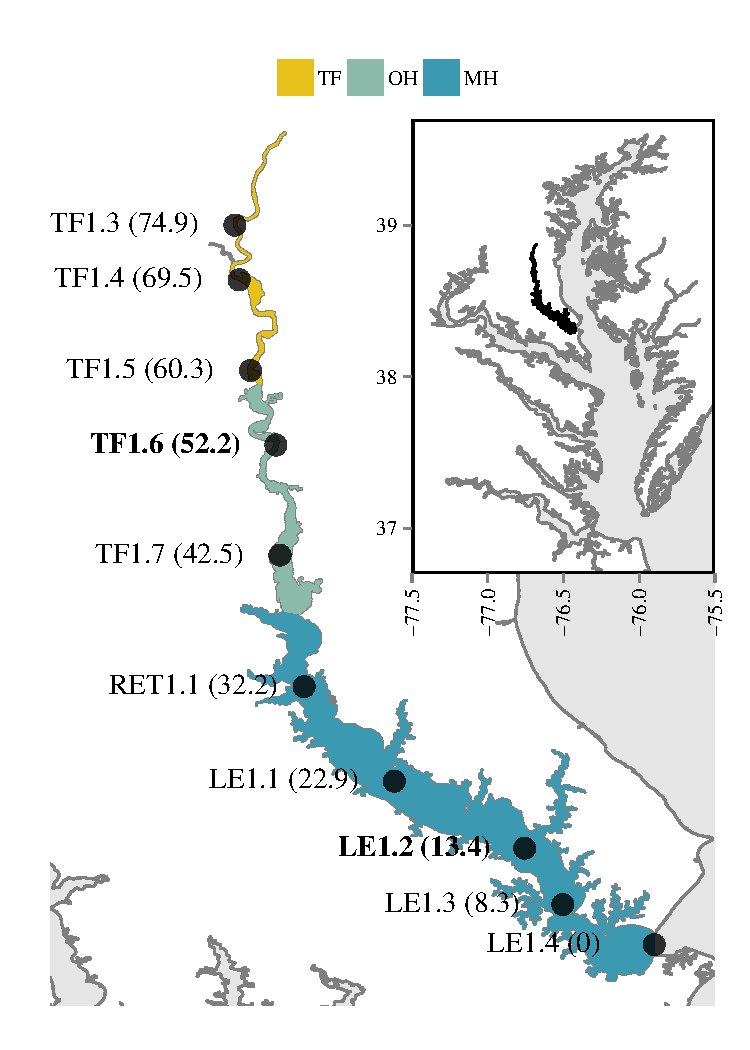
\includegraphics[width=0.7\textwidth]{figs/map-1} 

}

\caption{Patuxent River estuary with Chesapeake Bay inset. Fixed locations monitored by the Chesapeake Bay Program at monthly frequencies are shown along the longitudinal axis with distance from the mouth (km).  Study sites are in bold. Salinity regions in the Patuxent for the larger Chesapeake Bay area are also shown (TF = tidal fresh, OH = oligohaline, MH = mesohaline). See \cref{tab:statsum} for a numeric summary of station characteristics.}\label{fig:map}
\end{figure}



% chlorophyll trends by year, month, flow, combined
\begin{figure}[!ht]

{\centering 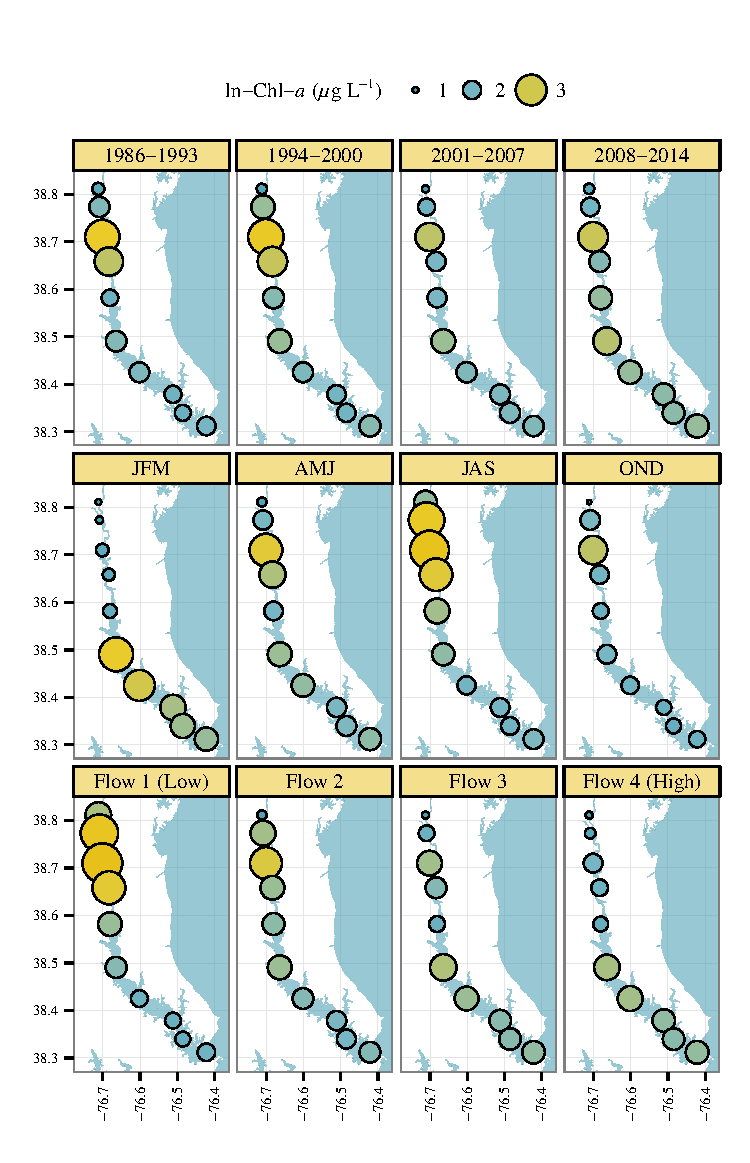
\includegraphics[width=\maxwidth]{figs/chlyrmofl-1} 

}

\caption{Annual, seasonal, and flow differences in chlorophyll trends at each monitoring station in the Patuxent River Estuary.  Size and color are proportional medians of ln-chlorophyll-a by year, season, and flow categories. See \cref{fig:map} for station numbers.}\label{fig:chlyrmofl}
\end{figure}



% predicted trends for each mod - monthly time series of observed with predictions, RMSE in fig


\begin{figure}
\centering
\subfloat[Monthly]{
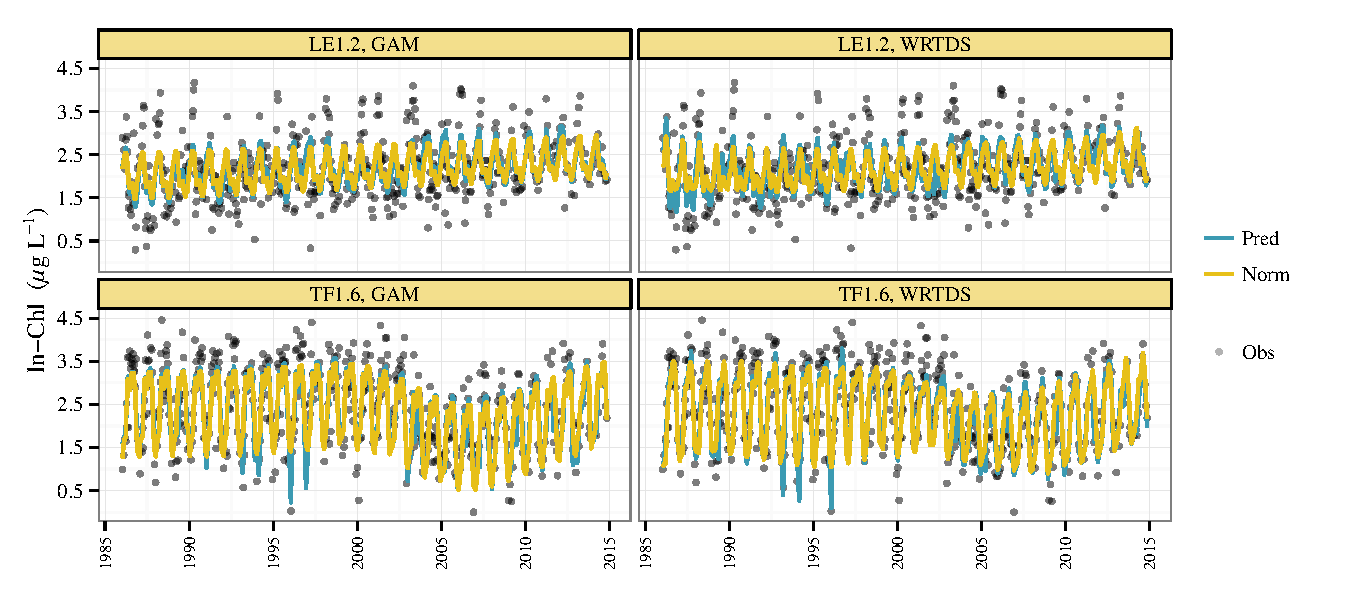
\includegraphics[width=\textwidth]{figs/predmo.pdf}
\label{fig:predmo}
}

\subfloat[Annual]{
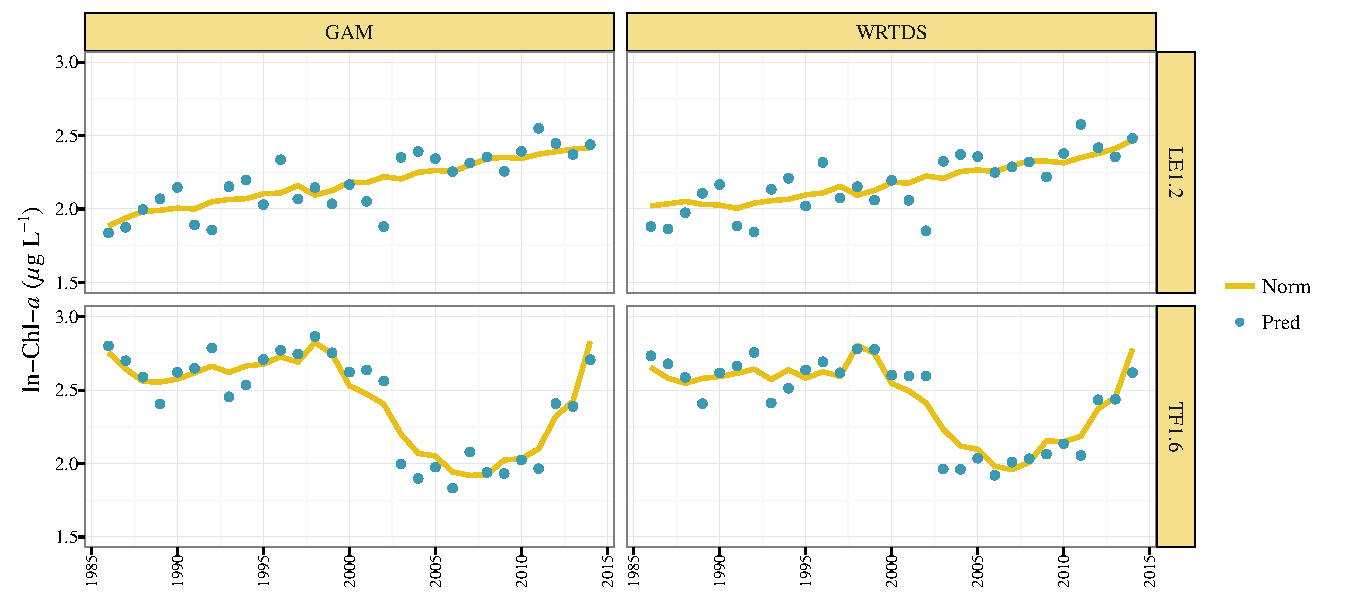
\includegraphics[width=\textwidth]{figs/predann.pdf}
\label{fig:predann}
}

\caption{Predicted chlorophyll from generalized additive models (GAM) and weighted regression (WRTDS) for LE1.2 and TF1.6 stations on the Patuxent River estuary.  \cref{fig:predmo} shows results at monthly time steps and \cref{fig:predann} shows results averaged by year.  Values in blue are model predictions and values in yellow are flow-normalized predictions.}
\label{fig:pred}
\end{figure}

% wrtds v gam predicions by periods
\begin{figure}[!ht]

{\centering 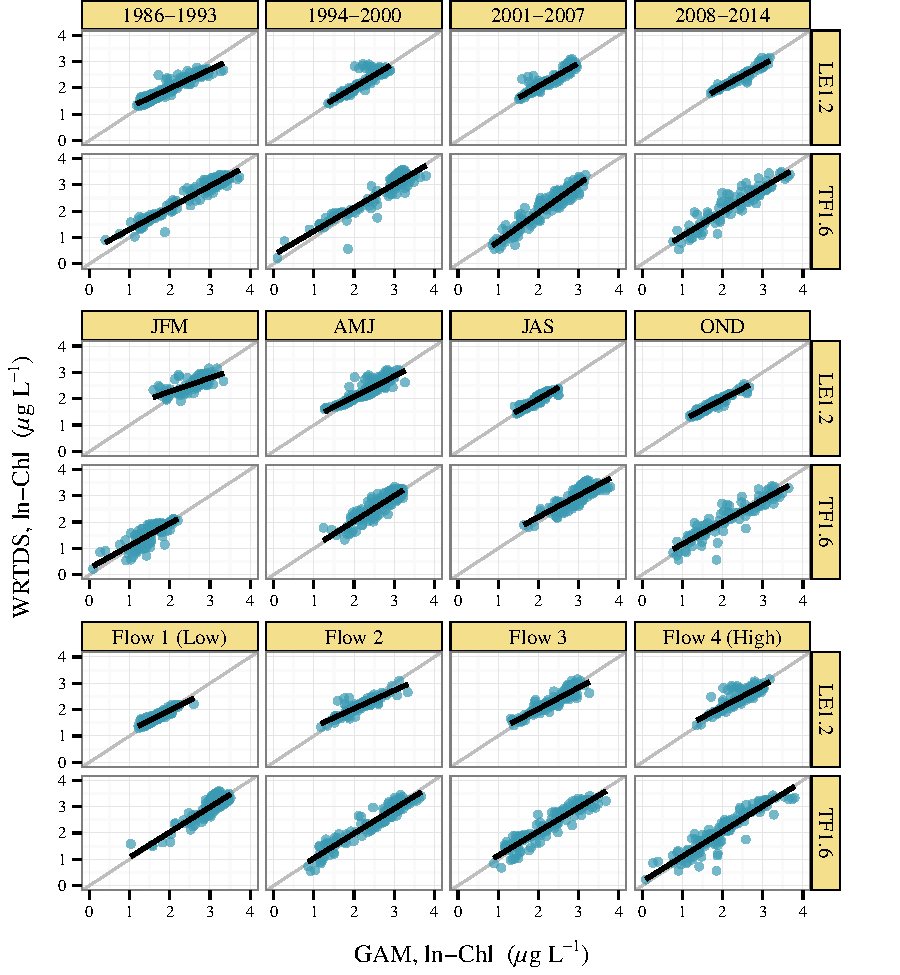
\includegraphics[width=\maxwidth]{figs/wrtdsvgam-1} 

}

\caption[Comparison of \ac{WRTDS} and \acp{GAM} predictions of \ac{chla} at each station (LE1]{Comparison of \ac{WRTDS} and \acp{GAM} predictions of \ac{chla} at each station (LE1.2, TF1.6) and different time periods.  Time periods are annual groupings every seven years (top), seasonal groupings by monthly quarters (middle), and flow periods based on quantile distributions from the discharge record (low).  Regression lines (thick black) and 1:1 replacement lines (thin grey) are also shown.}\label{fig:wrtdsvgam}
\end{figure}



% dynaplots for each mod (as in Fig. 8 Beck and Hagy 2015)

% examples of simulated datasets for eval of flow-normalization - daily, monthly, different flow effects

% results of flow-normalized data for simulations

\end{document}
